\section{重力}\label{sec:2-2}

河里的水总是从高处流向低处。手里拿着的书,脱手后就会落向地面。沿着任何方向扔出去的石头,最后也都会落到地面上来。
总之,一切物体,如果没有东西支持着它,都会向地面降落。这是为什么呢?
原来地球对地面附近的一切物体都有吸引作用,这种吸引作用要把一切物体拉向地面。
这种\textbf{由于地球的吸引而使物体受到的力叫做重力}。

\begin{wrapfigure}[12]{r}{4cm}
    \centering
    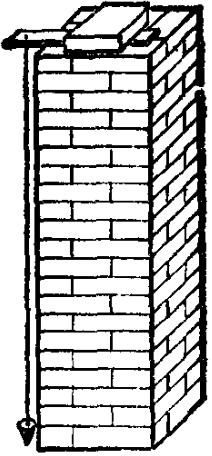
\includegraphics[width=0.15\textwidth]{../pic/czwl1-ch2-4}
    \caption{重垂线}\label{fig:2-4}
\end{wrapfigure}

为了叙述简便,我们常常把物体受到的重力说成物重。

根据经验知道,物体受到的重力是有大小的。一块大石头比一个小石子重,一大块铁比一个小铁钉重。
而大石头的质量比小石子的质量大,大铁块的质量比小铁钉的质量大。
可见,物体的质量越大,它就越重。
实际上,物体受到的重力跟它的质量是成正比的,质量增大到几倍,受到的重力也增大到几倍。
10 千克苹果是 1 千克苹果重的 10 倍。因此,你买的苹果越多,提在手里就觉得越重。

重力是有方向的。悬挂物体的绳子,静止时总是竖直下垂。这表明,重力的方向总是竖直向下的。
利用重力的这种性质,人们常在一根线的下端挂上一个重物,做成重垂线。
建筑房屋时可以用它来检查墙壁是否竖直(图 \ref{fig:2-4})。

重力对我们非常重要。如果没有重力,河水就不能流动,茶杯里的水就倒不进嘴里,飞扬的尘土就永远停留在空气中,
人轻轻一跳就会离开地球,扔出去的东西就回不到地面上来。总之,世界和我们的生活就都要改变样子了。

\lianxi

\begin{wrapfigure}[7]{r}{5cm}
    \centering
    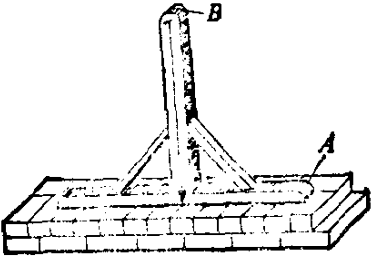
\includegraphics[width=0.25\textwidth]{../pic/czwl1-ch2-5}
    \caption{水平器}\label{fig:2-5}
\end{wrapfigure}

(1) 踢球时脚有什么感觉?为什么会有这种感觉?

(2) 游泳时用手和脚向后划水,人就前进。这是为什么?

(3) 物体受到的重力是什么物体施加的?

(4) 提在手里的水桶受到哪几个力的作用?哪个物体是受力物体?哪些物体是施力物体?

(5) 图 \ref{fig:2-5} 是一个水平器。$A$ 是一个刨得很平的木扳,$B$ 是垂直固定在 $A$ 上的木棒,上面刻着跟木板 $A$ 垂直的直线,
在这条直线的顶端挂着一根重垂线。怎样用这个水平器来检查桌面或窗台是否水平?

(6) 自己用螺丝帽做个重垂线,用它来检查门框、窗框、桌子腿等是否竖直。

